\documentclass[11pt,oneside]{article}
\usepackage[utf8]{inputenc}
\usepackage[a4paper,top=2cm,left=2cm,right=2cm,bottom=2cm]{geometry}
\usepackage{import}
\usepackage[T1]{fontenc}
\usepackage[german,ngerman]{babel}
\usepackage[table]{xcolor}
\usepackage{amsthm, esvect}
\usepackage{mathtools}
\RequirePackage{amssymb, amsfonts, amsmath, latexsym, verbatim, xspace}
\usepackage{systeme}
\usepackage{multicol}
\usepackage{multirow}
\usepackage{framed}
\usepackage{array}
\usepackage{ragged2e}
\usepackage{graphicx}
\usepackage{pdflscape}
\usepackage{epstopdf}
\usepackage{booktabs}
\usepackage{pdfpages}
\usepackage{float} % Allows putting an [H] in \begin{figure} to specify the exact location of the figure
\usepackage{wrapfig} % Allows in-line images such as the example fish picture
\usepackage{tikz, graphicx} % tikz
\usepackage[position=top]{subfig}
\usepackage[bookmarks=true]{hyperref}%Links
\usepackage{enumerate}
\usepackage{enumitem}
\usepackage[german,ruled,vlined,linesnumbered,algosection]{algorithm2e}
\usepackage[labelfont=sf]{caption}
\usepackage{lmodern}
\usepackage{lscape}
\usepackage{tabularx}
\usepackage{systeme}
\usepackage{hhline}
\usepackage{subfiles}
\usepackage{stackengine}
\usepackage{setspace}
\usepackage{MnSymbol}
\usepackage{tcolorbox}
\usepackage{bbm}
\usepackage{url}
\usepackage{xparse}
\usepackage{sectsty}
\usepackage{array}
\usepackage{ragged2e}
\usepackage{listings} %Stellt Code-Snippets sauber dar

% definiert die Sprache
\selectlanguage{German}

% add command for different dates in Swiss fashion
\newcommand{\monthwordlong}[1]{\ifcase#1 \or Januar\or Februar\or März\or April\or Mai\or Juni\or Juli\or August\or September\or Oktober\or November\or Dezember\fi}
\newcommand{\monthwordshort}[1]{\ifcase#1\or Jan\or Feb\or Mar\or Apr\or Mai\or Jun\or Jul\or Aug\or Sept\or Okt\or Nov\or Dez\fi}
\newcommand{\datelong}{\number\day.\:\monthwordlong{\the\month}\:\number\year}
\newcommand{\dateshort}{\number\day.\:\monthwordshort{\the\month}\:\number\year}

% define color of links inside a text
\definecolor{linkblue}{RGB}{0, 0, 80}
\definecolor{plotblue}{RGB}{100, 100, 255}
\definecolor{myblue}{RGB}{8,164,214}
\definecolor{myred}{RGB}{143,42,41}
\definecolor{forestgreen}{RGB}{34,139,34}
\definecolor{highdive}{RGB}{10,169,194}
\definecolor{charcoal}{RGB}{74,74,74}
\hypersetup{
	colorlinks=true,
	linkcolor=linkblue,
	filecolor=magenta,
	urlcolor=plotblue,
	citecolor=linkblue,
	pdfpagemode=FullScreen,
}


\lstdefinestyle{mystyle}{ % definiert den style des Code-Snippets
	%backgroundcolor=\color{backcolour},
	%commentstyle=\color{codegreen},
	%keywordstyle=\color{magenta},
	%numberstyle=\tiny\color{codegray},
	%stringstyle=\color{codepurple},
	basicstyle=\ttfamily\footnotesize,
	breakatwhitespace=false,
	breaklines=true,
	captionpos=b,
	keepspaces=true,
	%numbers=left,
	%numbersep=5pt,
	showspaces=false,
	showstringspaces=false,
	showtabs=false,
	tabsize=4
}
\lstset{style=mystyle}
\usepackage{fancyhdr}

\tcbuselibrary{breakable,skins}
\usetikzlibrary{mindmap,trees}
\newlength\tindent
\setlength{\tindent}{\parindent}
\setlength{\parindent}{0pt}
\renewcommand{\indent}{\hspace*{\tindent}}

\makeatletter
\def\ifEmpty#1{\def\@temp{#1}\ifx\@temp\@empty}
\makeatother

\sectionfont{\underline}
\usetikzlibrary{arrows, petri, topaths, graphs}


% =================== BEISPIEL ====================
\theoremstyle{definition}
\newtheorem{beispiel}{Beispiel}
\renewcommand{\thebeispiel}{\arabic{beispiel}}

% =================== AUFGABE =====================
\newcounter{aufg}[section] % Zähler für die Umgebungen

\newenvironment{aufgabe}[1][]{%
    \refstepcounter{aufg}% Inkrementiere den Zähler
    \begin{tcolorbox}[%
        enhanced,
        overlay unbroken and first={\mytitleaufg[#1]}, % Titelleiste mit Icons wird nicht über Seite gebrochen
        colframe=black,
        boxrule=0pt,
        breakable,
        top=15pt,
        before=\vskip18pt,
    ]
}{%
    \end{tcolorbox}
}

\newcommand{\mytitleaufg}[1][]{% Definiert die Titelleiste und Icons
    \node[fill=black!20,
        rounded corners,
        draw=black,
        text=black,
        line width=1pt,
        inner sep=4pt,
        anchor=west,
        xshift=12pt]
        at (frame.north west){\bfseries Aufgabe \thesection.\theaufg.\ifEmpty{#1}\else\emph{ (#1)}\fi}; % Titel, letzter Teil mit ifempty testet ob #1 leer und macht Klammern und Titel, falls Titelargument übergeben wird bzw. falls #1 leer erscheint nichts - auch keine Klammern

    \node[% Icon
        rounded corners,
        text=black,
        fill=black,
        line width=0pt,
        inner sep=3pt,
        anchor=west,
        xshift=5pt,
        % yshift=-35pt
        ]
        at (frame.north east){
\includegraphics[width=24pt]{../../../Header/Icons/aufgabeicon.png}};
}

% =================== DEFINITION ==================
\newcounter{def}[section] % Zähler für die Umgebungen

\newenvironment{definition}[1][]{%
    \refstepcounter{def}% Inkrementiere den Zähler
    \begin{tcolorbox}[%
        enhanced,
        drop shadow southeast,
        overlay unbroken and first={\mytitledef[#1]}, % Titelleiste mit Icons wird nicht über Seite gebrochen
        colback=blue!5!white,
        colframe=blue!75!black,
        boxrule=2pt,
        breakable,
        top=15pt,
        before=\vskip18pt,
    ]
}{%
    \end{tcolorbox}
}

\newcommand{\mytitledef}[1][]{% Definiert die Titelleiste und Icons
    \node[fill=blue!40!white,
        rounded corners,
        draw=black,
        text=black,
        line width=1pt,
        inner sep=4pt,
        anchor=west,
        xshift=12pt]
        at (frame.north west){\bfseries Definition \thesection.\thedef.\ifEmpty{#1}\else\emph{ (#1)}\fi}; % Titel, letzter Teil mit ifempty testet ob #1 leer und macht Klammern und Titel, falls Titelargument übergeben wird bzw. falls #1 leer erscheint nichts - auch keine Klammern

    \node[% Icon
        rounded corners,
        text=black,
        fill=black,
        line width=0pt,
        inner sep=3pt,
        anchor=west,
        xshift=5pt,
        % yshift=-35pt
        ]
        at (frame.north east){
\includegraphics[width=24pt]{../../../Header/Icons/definitionicon.png}};
}

% =================== NOTATION ====================
\newcounter{nota}[section] % Zähler für die Umgebungen

\newenvironment{notation}[1][]{%
    \refstepcounter{nota}% Inkrementiere den Zähler
    \begin{tcolorbox}[%
        enhanced,
        drop shadow southeast,
        colback=yellow!5!white,
        colframe=yellow!75!black,
        overlay unbroken and first={\mytitlenota[#1]},   % Titelleiste mit Icons wird nicht über Seite gebrochen
        boxrule=2pt,
        breakable,
        top=15pt,
        before=\vskip18pt,
    ]
}{%
    \end{tcolorbox}
}

\newcommand{\mytitlenota}[1][]{% Definiert die Titelleiste und Icons
    \node[fill=yellow!40!white,,
        rounded corners,
        draw=black,
        text=black,
        line width=1pt,
        inner sep=4pt,
        anchor=west,
        xshift=12pt]
        at (frame.north west){\bfseries Notation \thesection.\thenota.\ifEmpty{#1}\else\emph{ (#1)}\fi}; % Titel, letzter Teil mit ifempty testet ob #1 leer und macht Klammern und Titel, falls Titelargument übergeben wird bzw. falls #1 leer erscheint nichts - auch keine Klammern

    \node[% Icon
        rounded corners,
        text=black,
        fill=black,
        line width=0pt,
        inner sep=3pt,
        anchor=west,
        xshift=5pt,
        % yshift=-35pt
        ]
        at (frame.north east){
\includegraphics[width=24pt]{../../../Header/Icons/definitionicon.png}};
}

% =================== SATZ ========================
\newcounter{satz}[section]  % creates a counter and resets it after each chapter

\newenvironment{satz}[1][]{   % Hauptbox mit Satz drin
    \refstepcounter{satz}
    \begin{tcolorbox}[%
        enhanced,
        colback=red!5!white,
        fuzzy halo=2mm with gray,
        colframe=red!75!black,
        overlay unbroken and first={\mytitlesatz[#1]},   % Titelleiste mit Icons wird nicht über Seite gebrochen
        boxrule=2pt,
        breakable,
        top=15pt,
        before=\vskip18pt,
    ]
}{%
    \end{tcolorbox}
}

\newcommand{\mytitlesatz}[1][]{                     % Macht Titelbox und Icons
   \node[fill=red!90!white,
      rounded corners,
      draw=black,,
      text=black,
      line width=1pt,
      inner sep=4pt,
      anchor=west,
      xshift=12pt]
   at (frame.north west){\bfseries Satz \thesection.\thesatz.\ifEmpty{#1}\else\emph{ (#1)}\fi};  % Titel, letzter Teil mit ifx testet ob #1 leer und macht Klammern und Titel, falls Titelargument übergeben wird bzw.  falls #1 leer erscheint nichts - auch keine Klammern

 \node[ % Icon
      rounded corners,
      text=black,
      fill=black,
      line width=0pt,
      inner sep=3pt,
      anchor=west,
      xshift=5pt,
%     yshift=-35pt
]
   at (frame.north east){ 
\includegraphics[width=24pt]{../../../Header/Icons/satzicon.png} };
}

% =================== BEWEIS ======================
\newenvironment{beweis}[1][]{
    \begin{tcolorbox}[
        enhanced,
        overlay unbroken and first={\mybeweis[#1]},     % Titelleiste mit Icons wird nicht über Seite gebrochen
        colback=white,
        colframe=black,
        boxrule=0pt,
        breakable,
        top=15pt,
        before=\vskip18pt,
    ]
}{
        \end{tcolorbox}
}

\newcommand{\mybeweis}[1][]{                     % Macht Titelbox und Icons
   \node[fill=white,
      rounded corners,
      draw=black,
      text=black,
      line width=1pt,
      inner sep=4pt,
      anchor=west,
      xshift=12pt]
   at (frame.north west){\bfseries Beweis \ifEmpty{#1}\else\emph{ (#1)}\fi};  % Titel, letzter Teil mit ifx testet ob #1 leer und macht Klammern und Titel, falls Titelargument übergeben wird bzw.  falls #1 leer erscheint nichts - auch keine Klammern
}

% =================== ALGORITHM ===================
\newcounter{algo}[section]  % creates a counter and resets it after each chapter

\newenvironment{algo}[1][]{   % Hauptbox mit Satz drin
    \refstepcounter{algo}
    \begin{tcolorbox}[%
        enhanced,
        drop shadow southeast,
        colback=yellow!5!white,
        colframe=yellow!75!black,
        overlay unbroken and first={\algotitle[#1]},   % Titelleiste mit Icons wird nicht über Seite gebrochen
        boxrule=2pt,
        breakable,
        top=15pt,
        before=\vskip18pt,
    ]
}{%
    \end{tcolorbox}
}

\newcommand{\algotitle}[1][]{                     % Macht Titelbox und Icons
   \node[fill=yellow!40!white,
      rounded corners,
      draw=black,
      text=black,
      line width=1pt,
      inner sep=4pt,
      anchor=west,
      xshift=12pt]
   at (frame.north west){\bfseries \ifEmpty{#1}{Ablauf}\else{#1}\fi};  % Titel, letzter Teil mit ifx testet ob #1 leer und macht Klammern und Titel, falls Titelargument übergeben wird bzw.  falls #1 leer erscheint nichts - auch keine Klammern

 \node[ % Icon
      rounded corners,
      text=black,
      fill=black,
      line width=0pt,
      inner sep=3pt,
      anchor=west,
      xshift=5pt
      % yshift=-35pt
      ]
   at (frame.north east){ 
\includegraphics[width=24pt]{../../../Header/Icons/algoicon.png} };
}

% ================ Nummerierte Multicol ================
\newenvironment{enumcols}[1][]{
    \begin{enumerate}[label=\alph*)]\begin{multicols}{#1}
}{
    \end{multicols}\end{enumerate}
}



% =================================================
\usetikzlibrary{shapes,arrows}
\tikzstyle{decision} = [diamond, draw, fill=blue!20,
    text width=6em, text badly centered, node distance=4cm, inner sep=0pt]
\tikzstyle{block} = [rectangle, draw, fill=blue!20,
    text width=8em, text centered, rounded corners, minimum height=4em]
\tikzstyle{line} = [draw, -latex']
\tikzstyle{cloud} = [draw, ellipse,fill=red!20, node distance=2cm,
    minimum height=2em]

% Karriertes Papier für Antwort
\newcommand{\karos}[1]{\begin{tikzpicture}\draw[step=0.5cm,color=gray] (0,0) grid (\linewidth,#1 cm);\end{tikzpicture}}
%%
% Header and Footer
%%
\linespread{1.2} % Line spacing
\fancypagestyle{plain}{
	\pagestyle{fancy}
	\lhead{}
	\chead{}
	\rhead{}
	\lfoot{\Autor}
	\cfoot{\Skriptname}
	\rfoot{\thepage}
	\renewcommand{\headrulewidth}{0pt}
	\renewcommand{\footrulewidth}{0.4pt}
}

\pagestyle{fancy}
\fancyhf{}
\rhead{\rightmark}
\lfoot{\leftmark}
\rfoot{\thepage}
\renewcommand{\headrulewidth}{0.2pt}
%\setlength\parindent{0pt} % Uncomment to remove all indentation from paragraphs



%%
% Math Arrows
%%
\newcommand{\same}{\ensuremath{\Longleftrightarrow}}
\renewcommand{\to}{\ensuremath{\longrightarrow}}
\newcommand{\qsame}{\quad\same\quad}
\newcommand{\dsame}{\ensuremath{:\Leftrightarrow}}
\newcommand{\qdsame}{\quad\dsame\quad}
\newcommand{\ldsame}{\ensuremath{:\Longleftrightarrow}}
\newcommand{\samedef}{\ensuremath{\us {\text{def}} \Leftrightarrow}}
\newcommand{\qsamedef}{\quad\samedef\quad}
\newcommand{\lsamedef}{\ensuremath{\us {\text{def}} \Longleftrightarrow}}
\newcommand{\qlsamedef}{\quad\lsamedef\quad}


%%
% Mengendefinitionen
%%
\newcommand{\M}{\ensuremath{\mathcal{M}}}
\newcommand{\N}{\ensuremath{\mathbb{N}}}
\newcommand{\Z}{\ensuremath{\mathbb{Z}}}
\newcommand{\Q}{\ensuremath{\mathbb{Q}}}
\newcommand{\I}{\ensuremath{\mathbb{I}}}
\newcommand{\R}{\ensuremath{\mathbb{R}}}
\newcommand{\C}{\ensuremath{\mathbb{C}}}
\renewcommand{\S}{\ensuremath{\mathbb{S}}}
\newcommand{\Prim}{\ensuremath{\mathbb{P}}}
\newcommand{\0}{\ensuremath{\emptyset}}
\renewcommand{\Re}{\ensuremath{\operatorname{Re}}}
\renewcommand{\Im}{\ensuremath{\operatorname{Im}}}
\newcommand{\strich}{\ensuremath{\big\vert}}

%%
% Mengenoperation
%%
\renewcommand{\nin}{\not\in}


%%
% Logisches Und und Oder
%%
\newcommand{\sand}{\ensuremath{\; \land \;}}
\newcommand{\sor}{\ensuremath{\; \lor \;}}
\renewcommand{\*}{\ensuremath{\cdot}}
\newcommand{\oder}{\vee}
\newcommand{\n}{\neg}
\newcommand{\und}{\wedge}


%%
% Bei Integral, Summe,... die Grenzen über bzw.
% unter das Zeichen
%%
\renewcommand{\d}[1]{\ensuremath{\operatorname{d}\!{#1}}}
\newcommand{\Sum}{\sum\limits}
\newcommand{\Prod}{\prod\limits}
\newcommand{\Min}{\min\limits}
\newcommand{\Max}{\max\limits}
\newcommand{\Lim}{\lim\limits}
\newcommand{\Inf}{\inf\limits}
\newcommand{\Sup}{\sup\limits}
\newcommand{\Liminf}{\liminf\limits}
\newcommand{\Limsup}{\limsup\limits}
%\renewcommand{\Cup}{\bigcup\limits}
%\renewcommand{\Cap}{\bigcap\limits}
\newcommand{\Otimes}{\bigotimes\limits}
\newcommand{\Oplus}{\bigoplus\limits}


%%
% Arcus Cotangens, Logarithmus
%%
\let\oldsin\sin
\renewcommand{\sin}[1]{\oldsin{\left(#1\right)}}
\let\oldcos\cos
\renewcommand{\cos}[1]{\oldcos{\left(#1\right)}}
\let\oldtan\tan
\renewcommand{\tan}[1]{\oldtan{\left(#1\right)}}
\let\oldarcsin\arcsin
\renewcommand{\arcsin}[1]{\oldarcsin{\left(#1\right)}}
\let\oldarccos\arccos
\renewcommand{\arccos}[1]{\oldarccos{\left(#1\right)}}
\let\oldarctan\arctan
\renewcommand{\arctan}[1]{\oldarctan{\left(#1\right)}}
\let\oldln\ln
\renewcommand{\ln}[1]{\oldln{\left(#1\right)}}
\newcommand{\Log}[2]{\ensuremath{\operatorname{log}_{#1}\left(#2\right)}}
\newcommand{\e}{\operatorname{e}}
\renewcommand{\exp}[1]{\ensuremath{\operatorname{\e}^{#1}}}


%%
% Griechische Buchstaben
%%
\renewcommand{\epsilon}{\ensuremath{\varepsilon}}
\renewcommand{\phi}{\varphi}
\renewcommand{\l}{\lambda}
\renewcommand{\t}{\tau}


%%
% Bezeichnungen
%%
\newcommand{\Rgn}{\R_{>0}} % R grösser Null
\newcommand{\Rad}{\operatorname{Rad}}   % Radikal
\newcommand{\kgV}{\operatorname{kgV}}   % Kleinster gemeinsame Vielfache
\newcommand{\ggT}{\operatorname{ggT}}   % Grösster gemeinsame Teiler
\newcommand{\winkel}{\sphericalangle}          % Winkelsymbol
\DeclarePairedDelimiter\abs{\lvert}{\rvert} % besserer Betrag
\makeatletter
\let\oldabs\abs
\def\abs{\@ifstar{\oldabs}{\oldabs*}}
\makeatother


%%
% Vektorgeometrie
%%
\renewcommand{\v}[1]{\vv{#1}}       % besserer Pfeil über Buchstaben
\renewcommand{\vec}[2]{\begingroup\renewcommand{\arraystretch}{1}\left(\begin{array}{c} #1 \\ #2 \end{array}\right)\endgroup}   % two dimensional vector
\renewcommand{\Vec}[3]{\begingroup\renewcommand{\arraystretch}{1}\left(\begin{array}{c} #1 \\ #2 \\ #3 \end{array}\right)\endgroup}      % three dimensional vector


%%
% Text
%%
\newcommand*{\Ueq}[1]{\mathrel{\mathop{=}\limits_{\text{#1}}}}
\newcommand*{\Oeq}[1]{\mathrel{\stackrel{\text{#1}}{=}}}
\newcommand{\utext}[2]{\underbrace{#1}_{\substack{#2}}}
\newcommand{\otext}[2]{$\overbrace{\textrm{#1}}^{\textrm{#2}}$}
\newcommand{\lineortext}[1]{\hspace{0,1cm}\underline{\hspace{0.1cm}\hphantom{#1}\hspace{0.1cm}}\hspace{0,1cm}} % Lückentext erstellen
\newcommand{\gap}[1]{\rule{#1 cm}{1pt}}
\graphicspath{{images/}}


\newcommand{\Skriptname}{Lineare Gleichungssysteme}
\newcommand{\Autor}{Jonas Guler (Gu)}
\newcommand{\version}{\textit{v}1.0}

\begin{document}   %KSH-Gubser - LATEX/PDF
\begin{titlepage}
	\clearpage
	\title{\Huge\textbf{\Skriptname} \\[1cm]}
	\author{Autor:\\ \Autor}
	\date{\normalsize {Version \version}\\ \datelong}
	\maketitle
	\thispagestyle{empty}
	\vfill
	\tableofcontents
\end{titlepage}
\pagenumbering{arabic}
%############################################################################################
\section{Einleitung}
	Mit diesen Unterlagen werden wir uns das Thema \flqq Gleichungssysteme\frqq\:erarbeiten. Mit Gleichungen können wir Probleme lösen, die aus den verschiedensten Bereichen kommen: aus der Mathematik selbst, aus der Technik, aus der Wirtschaft. Es gibt auch Aufgaben, die von Menschen allein zur Unterhaltung gelöst werden (Knobelaufgaben). Bei all diesen Problemen haben wir Grössen, die zwar unbekannt sind, über die wir jedoch einiges wissen.\newline
	1973 hat eine neue Technik die medizinische Diagnostik revolutioniert. Diese Diagnosetechnik heisst Computer-Tomographie. Sie stützt sich auf Röntgenstrahlen, lineare Gleichungssysteme und Computer. Beim herkömmlichen Röntgen werden ganze Körperpartien durchleuchtet. Bei der Computer-Tomographie hingegen werden Röntgenstrahlen nur durch eine schmale Schicht des Körpers geschickt. Messungen und Computerberechnungen liefern dann ein Bild dieser Körperschicht, ein sogenanntes Tomogramm.
	\begin{figure}[H]
		\centering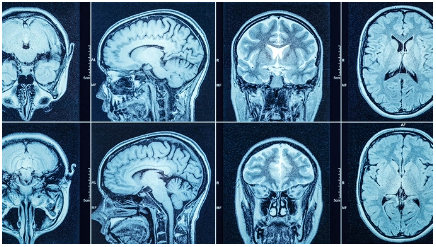
\includegraphics[scale=0.6]{tomogramm.png}
	\end{figure}
	Lasst uns zuerst mit einem bekannten Rätsel beginnen:
	\begin{aufgabe}
		Franz und Marie zählen ihr Taschengeld. Franz sagt: Wenn du mir $1$ Franken gibst, dann habe ich doppelt so viel wie du. Darauf erwidert Marie: Gib du mir lieber $1$ Franken, dann haben wir beide gleich viel.  –  Wie viel Taschengeld besitzen beide?\vspace{5pt}\newline\karos{8}
	\end{aufgabe}
	\begin{definition}
		Ein lineares $2\times2$ Gleichungssystem besteht aus zwei linearen Gleichungen mit je zwei Variablen $x,y$:
		\[\systeme*{a\*x + b\*y = n_1,c\*x + d\*y = n_2}\]
		Die Parameter $a,b,c,d,n_1,n_2\in\R$ sind reele Zahlen und werden als \textbf{Koeffizienten} des Gleichungssystems bezeichnet. Die Lösung eines linearen $2\times2$ Gleichungssystems ist ein Zahlenpaar $\left(x_0|y_0\right)$, sodass beide Gleichungen erfüllt sind.
	\end{definition}
	Selbstverständlich gibt es auch lineare $3\times3,\:4\times4,\:\text{etc.}$ Gleichungssysteme. Ganz allgemein kann also auch von einem $m\times n$ Gleichungssystem gesprochen werden. Im folgenden werden wir uns zuerst auf lineare $2\times2$ Gleichungssysteme beschränken und uns mit verschiedenen Lösungsmethoden für solcher befassen. Bevor wir starten, sollen zwei Punkte festgehalten werden:
	\begin{itemize}
		\item Eine Gleichung mit den Unbekannten $x$ und $y$, so wie wir sie erhalten haben, allgemein: eine Gleichung, die sich auf die Form $ax + by = c$ bringen lässt (mit reellen Zahlen $a,b,c\in\R$), heisst \textbf{linear}.
		(Die Unbekannten kommen darin also weder quadratisch oder in höheren Potenzen noch miteinander multipliziert vor.)
		\item 	Eine einzige lineare Gleichung mit mehreren Unbekannten hat im Allgemeinen unendlich viele Lösungen.\newline
		Betrachten wir z.B. nochmals die zweite Gleichung von oben, x - y  =  2, die Maries Aussage übersetzt: Gib mir 1 Franken, dann haben wir beide gleich viel. Sie besagt einfach, dass Franz 2 Franken mehr besitzt als Marie. Wenn wir nur das wüssten, dann gäbe es unendlich viele Lösungsmöglichkeiten, z.B.: $x = 3,y = 1$ oder $x = 4,y = 2$ oder $x = 5,y = 3$, usw.\newline
		Wenn das Problem eine eindeutige Lösung haben soll, braucht es eine weitere Information, aus der wir eine weitere Gleichung gewinnen können. (Hier ist es die Aussage von Franz, die zur ersten Gleichung geführt hat.)
	\end{itemize}
	\begin{satz}
		Damit ein System von linearen Gleichungen eine \textbf{eindeutige Lösung} besitzt, braucht es mindestens so viele Gleichungen wie Unbekannte.
	\end{satz}
	\begin{beispiel}
		Bringe das lineare $2\times2$ Gleichungssystem in die Standardform wie in obiger Definition.
		\[\systeme*{5x-7=3y+2,x+3y=5-4x}\hspace*{12cm}\]
		\karos{4}
	\end{beispiel}
	\begin{aufgabe}
		\begin{enumerate}
			\item Bringe die linearen $2\times2$ Gleichungssysteme in die Standardform und lese die Werte der Koeffizienten ab.
			\begin{enumcols}[2]
				\item $\displaystyle\systeme*{5x-4y=8y+\frac{2}{5}x,3(y-4)=-11+5y}$
				\item $\displaystyle\systeme*{2x-5=\frac{4y+1}{3},3(2x+2)=3y+6}$
			\end{enumcols}
			\item Überprüfe, ob die folgenden Zahlenpaare eine Lösung des jeweiligen linearen $2\times2$ Gleichungssystems sind.
			\begin{enumcols}[2]
				\item $\displaystyle\systeme{x+y=10,x-y=9}\quad,\left(x_0|y_0\right)=\left(9.5|0.5\right)$
				\item $\displaystyle\systeme{2x+y=-1,x+2y=5}\quad,\left(x_0|y_0\right)=\left(2|3\right)$
				\item $\displaystyle\systeme{4x-3y=11,6x+y=1}\quad,\left(x_0|y_0\right)=\left(0.5|-3\right)$
				\item $\displaystyle\systeme{4x+3y=10,6x+y=8}\quad,\left(x_0|y_0\right)=\left(1|2\right)$
			\end{enumcols}
			\item Stelle ein lineares $2\times2$ Gleichungssystems auf, welches die folgenden Lösungen besitzt.
			\begin{enumcols}[3]
				\item $\left(x_0|y_0\right)=\left(1|1\right)$
				\item $\left(x_0|y_0\right)=\left(2|-5\right)$
				\item $\left(x_0|y_0\right)=\left(0|2.5\right)$
			\end{enumcols}
		\end{enumerate}
	\end{aufgabe}
	\newpage


\section{Graphische Lösung von linearen Gleichungssystemen}
	Für lineare $2\times2$ Gleichungssysteme kann die Lösung auf eine sehr elegante Weise auch graphisch interpretiert werden. Dabei wird hoffentlich auch ersichtlich, welche Spezialfälle beim im Lösungsverfahren auftauchen können. Betrachten wir also zunächst folgendes lineares $2\times2$ Gleichungssystem:
	\[\systeme{2x-3y=9,x+2y=8}\]
	Die Lösung dieses Gleichungssystems ist also ein Zahlenpaar bestehend aus zwei reellen Zahlen. Mit Hilfe einfacher algebraischer Umformungen können die Gleichungen im obigen System beide nach $y$ aufgelöst werden:
	\[\systeme{y=\frac{2}{3}x-3,y=-\frac{1}{2}x+4}\]
	Diese Gleichungen können wir nun als Funktionsgleichungen von zwei verschiedenen linearen Funktionen auffassen. Dementsprechend sind wir in der Lage, diese Geraden in einem Koordinatensystem graphisch darzustellen.
	\begin{figure}[H]
		\centering
		\begin{tikzpicture}[cross/.style={draw, cross out, minimum size=2*(#1-1pt), inner sep=0pt, outer sep=0pt}, x=10mm, y=10mm,
			>=latex,   %Voreinstellung für Pfeilspitzen
			font=\footnotesize, scale=0.8]
			%Raster zeichnen
			\draw [color=gray!50]  [step=10mm] (-4.3,-3.3) grid (8.3,6.3);
			% Achsen zeichnen
			\draw[->,thick] (-4.3,0) -- (8.7,0) node[right, below] {\normalsize $x$};
			\draw[->,thick] (0,-3.3) -- (0,6.7) node[above, left] {\normalsize $y$};
			% Achsen beschriften
			\foreach \x in {-4,...,-2,-1,1,2,...,8} \draw (\x,-.1) -- (\x,.1) node[below=5pt, xshift=4pt] {$\x$};
			\foreach \y in {-3,-2,-1,1,2,...,6} \draw (-.1,\y) -- (.1,\y) node[left=5pt, yshift=2pt] {$\y$};
			% Besserer Ursprung
			\draw[color=black] (0.3,-0.4) node {$0$};
			%Funktionen zeichnen:
			\clip(-0.3,-0.3) rectangle (5.3,5.3); %Bildbereich
			%Beschriftung
			%\node[blue]  at (11,5) {\normalsize$f$};
		\end{tikzpicture}
	\end{figure}
	Die Zahlenpaare $\left(x_0|y_0\right)$, welche die erste Gleichung lösen, sind die Koordinaten aller Punkte, die auf der einen Gerade liegen. Gleiches gilt für die zweite Gleichung resp. die zweite Gerade.\newline
	Jedoch suchen wir das Zahlenpaar, welches beide Gleichungen gleichzeitig löst, denn dieses entspricht der Lösung des linearen $2\times2$ Gleichungssystems.\vspace*{5pt}\newline\karos{3.5}
	\begin{satz}[Graphische Lösungsmethode]
		Ist ein lineares $2\times2$ Gleichungssystem gegeben, können die Graphen der Geraden mit Hilfe der Funktionsgleichungen in ein Koordinatensystem gezeichnet werden. Die Lösung des Gleichungssystems können aus den Koordinaten \gap{5} abgelesen werden.
	\end{satz}
	Gemäss dem obigen Koordinatensystem ist die eindeutige Lösung des Gleichungssystems also \[\gap{5}.\]
	\begin{aufgabe}
		\begin{enumerate}
			\item Löse die folgenden lineare $2\times2$ Gleichungssysteme, in dem du die zugehörigen Geraden in ein Koordinatensystem mit $-3\leq x\leq 5$ und $-4\leq y\leq 7$ einzeichnest.
			\begin{enumcols}[4]
				\item $\displaystyle\systeme{x-2y=2,x+y=3}$
				\item $\displaystyle\systeme{x+3y=9,-x+9y=15}$
				\item $\displaystyle\systeme{4x+3y=11,x-2y=0}$
				\item $\displaystyle\systeme{9x-2y=4,11x+y=29}$
			\end{enumcols}
			\item Zeichne als nächstes die Geraden der folgenden beiden linearen Gleichungssystemen in ein Koordinatensystem ein. Was kannst du daraus, über die Lösung aussagen?
			\begin{enumcols}[2]
				\item $\displaystyle\systeme*{3x-5=7-2y,-y-3x=y-12}$
				\item $\displaystyle\systeme*{5x-4=10-y,10x+2y=6}$
			\end{enumcols}
			\item Woran erkennst den Unterschied in den Lösungen auch rechnerisch?
			\item Erfinde ein lineares $2\times2$ Gleichungssystem, das keine Lösung besitzt.
			\item Erfinde ein lineares $2\times2$ Gleichungssystem, das unendlich viele Lösungen besitzt.
		\end{enumerate}
	\end{aufgabe}
	\newpage

\section{Rechnerische Lösungsmethoden}
	Bleiben wir für den Moment bei linearen $2\times2$ Gleichungssystemen; also zwei Gleichungen und zwei Unbekannten.\vspace*{11pt}\newline
	Die allgemeine Strategie zur Lösung lautet:\newline
	Man versucht, aus einem solchen System eine Gleichung zu gewinnen, die nur noch eine Unbekannte enthält. Man muss also dazu die andere Variable eliminieren (lat. eliminare = beseitigen).\vspace*{11pt}\newline
	Dies kann durch verschiedene Verfahren erreicht werden, die alle (je nach Problemtyp) wichtig sind.

\subsection{Das Gleichsetzungsverfahren}
	Dieses Verfahren kennen wir von der Berechnung des Schnittpunkts zweier Geraden (siehe wieder \flqq lineare Funktionen\frqq).
	Wir betrachten nochmals das Beispiel aus der geometrsichen Betrachtung.
	\begin{align*}
		\systeme{2x-3y=9,x+2y=8}
	\end{align*}
	Durch geeignetes algebraischen Umformen können beiden Gleichungen nach derselben Variablen (entweder nach $y$ oder nach $x$) aufgelöst werden.So erhalten wir die Gleichungen:
	\begin{align*}
		\systeme{y=\frac{2}{3}x-3, y=-\frac{1}{2}x+4}
	\end{align*}
	So haben wir zwei unterschiedliche Terme erhalten, welche beide die Variable $y$ beschreiben. Gleichsetzen dieser Terme liefert und eine einzige Gleichung in $x$, die sich leicht lösen lässt: \vspace*{5pt}\newline\karos{5}
	Zum Schluss berechnen wir die zweite Variable $y$, in dem wir das Resultat für $x=6$ in eine der obigen Gleichungen einsetzen\vspace*{5pt}\newline\karos{2.5}
	Zusammenfassend kann das Vorgehen also folgendermassen beschrieben werden:
	\begin{algo}[Gleichsetzungsverfahren]
		\begin{enumerate}[label=\Roman*)]
			\item Löse beide Gleichungen nach derselben Variablen auf.
			\item Setze die beiden erhaltenen Gleichungen gleich und löse nach der verbleibenden Variable auf.
			\item Bestimme die zweite Variable durch Einsetzen in eine der beiden Gleichungen.
		\end{enumerate}
	\end{algo}
	\begin{beispiel}
		Lasst uns gemeinsam ein zweites Beispiel lösen. Dazu betrachten wir das folgende lineare Gleichungssystem.
		\[\systeme{-2y+3=5x-1,-2y+3=-8x}\hspace*{12cm}\]\karos{10}
	\end{beispiel}
	\begin{aufgabe}
		\begin{enumerate}
			\item Löse die folgenden linearen $2\times2$ Gleichungssysteme mit Hilfe des Gleichsetzungsverfahren.
			\begin{enumcols}[4]
				\item $\displaystyle\systeme{2x-6y=6,5x+3y=42}$
				\item $\displaystyle\systeme{3x-10y=3,-9x+24y=-10}$
				\item $\displaystyle\systeme{\frac{1}{2}x-3y=-6,-2x+3y=\frac{3}{2}}$
				\item $\displaystyle\systeme{3x+9y=12,9x+3y=4}$
			\end{enumcols}
			\item Löse auch das folgende lineare $2\times2$ Gleichungssystem. Denk daran, du kannst auch ganze Terme gleichsetzen.
			\[\systeme*{2(5x-2)=\frac{2y+8}{3},10x-4=y+1}\hspace*{10.5cm}\]
		\end{enumerate}
	\end{aufgabe}
	\newpage

\subsection{Das Einsetzungsverfahren (auch Substitutionsverfahren)}
	Bevor wir mit einem Beispiel starten, lasst uns direkt erste Lösungsversuche machen und die Methode selbstständig herleiten.
	\begin{aufgabe}
		\begin{enumerate}
			\item Versuche nacheinander die folgenden linearen Gleichungssysteme zu lösen:
			\begin{enumcols}[4]
				\item $\displaystyle\systeme{2x+3y=9,y=2}$
				\item $\displaystyle\systeme{5x+2y=22,\frac{y}{2}=3}$
				\item $\displaystyle\systeme{3x+5y=20,y=x}$
				\item $\displaystyle\systeme{2x+3y=13, y=x+1}$
				\item $\displaystyle\systeme{4x-3y=6,2y=x-2}$
				\item $\displaystyle\systeme{11x-7y=5,-x+y=0}$
				\item $\displaystyle\systeme{6x+8y,x+y=5}$
				\item $\displaystyle\systeme{2x+3y=4,3x+2y=2}$
			\end{enumcols}
		\end{enumerate}
		\karos{12.5}
		\begin{enumerate}
			\setcounter{enumi}{1}
			\item Erkläre, wie du oben vorgegangen bist.
		\end{enumerate}
		\karos{2.5}
	\end{aufgabe}
	\begin{algo}[Einsetzungsverfahren)]
		Lasst uns die einzelnen Schritte am Beispiel des folgenden Gleichungssystem beschreiben:
		\[\systeme{2x-5y=7,3x+2y=1}\]
		\karos{6.5}
	\end{algo}
	Du kannst lineare Gleichungssysteme auch mithilfe des Solvers des TI-Nspire lösen:\vspace{11pt}\newline
	Der Taschenrechner ist zwar sehr bequem, wir wollen jedoch auch ein wenig Routine haben, Gleichungssysteme von Hand zu lösen. Obwohl es Autos, Bahnen und Flugzeuge gibt, sollte man doch auch zu Fuss gehen können.
	\begin{aufgabe}
		\begin{enumerate}
			\item Löse die folgenden Gleichungssysteme mit Hilfe des Einsetzungsverfahren.
			\begin{enumcols}[3]
				\item $\displaystyle\systeme{x+y=11,-x+y=87}$
				\item $\displaystyle\systeme{x_1+2x_2=5, 4x_1+6x_2=10}$
				\item $\displaystyle\systeme{4u-5v=1, 5v-9u=1}$
				\item $\displaystyle\systeme{0.2x+0.6y=2, 0.3x+0.8y=1}$
				\item $\displaystyle\systeme{8x-7y=9,-2x+3y=2}$
				\item $\displaystyle\systeme{6x-y=12,3.8x+0.4y=1.4}$
				\item $\displaystyle\systeme{\frac{1}{3}x-\frac{1}{5}y=8,\frac{1}{5}x+\frac{1}{3}y=-2}$
				\item $\displaystyle\systeme{x+\frac{1}{3}y=4,\frac{3}{5}x-\frac{2}{3}y=5}$
				\item $\displaystyle\systeme{2x-\frac{6}{4}y+\frac{28}{4}=12, \frac{2}{9}x-\frac{1}{3}y+\frac{5}{9}=2}$
			\end{enumcols}
			\item Gegeben ist das Gleichungssystem \[\systeme{\frac{1}{4}x-4y=0,x+8y=3}\] Welche der drei folgenden Lösungsansätze sind richtig, welche falsch? Rechne die richtigen Ansätze fertig.\newline
			\begin{enumerate}[label=\alph*)]
				\item Alice geht beim Lösen so vor: \[\systeme{\frac{1}{4}x-4y=0,x+8y=3}\Leftrightarrow\systeme*{\frac{1}{4}x-4y=0,x=3-8y}\Leftrightarrow \frac{1}{4}\*(3-8y)-4y=0\Leftrightarrow\ldots\]
				\item Bruno geht beim Lösen so vor: \[\systeme{\frac{1}{4}x-4y=0,x+8y=3}\Leftrightarrow\systeme*{x-16y=0,x=3-8y}\Leftrightarrow (3-8y)-16y=0\Leftrightarrow\ldots\]
				\item Carla geht beim Lösen so vor: \[\systeme{\frac{1}{4}x-4y=0,x+8y=3}\Leftrightarrow\systeme*{\frac{1}{4}x=4y,x+2\*4y=3}\Leftrightarrow x+2\*\frac{1}{4}x=3\Leftrightarrow\ldots\]
			\end{enumerate}
		\end{enumerate}
	\end{aufgabe}
	\newpage


\subsection{Das Additionsverfahren}
	Betrachten wir schliesslich noch das sogenannte Additionsverfahren. Bei diesem Verfahren handelt es sich um das für uns wichtigste, wenn es darum geht, lineare Gleichungssysteme zu lösen. Hierbei müssen wir nicht nach einer Variable auflösen.
	\begin{beispiel}
		Betrachten wir zunächst wieder ein Beispiel:
		\begin{align*}
			\systeme{x-4y=8, 3x+4y=12}
		\end{align*}
		Beide Gleichungen: I: $x-4y=8$ und II: $3x+4y=12$ können wir als Waage veranschaulichen, welche im Gleichgewicht ist.\newline
		\begin{minipage}{0.45\linewidth}
			\centering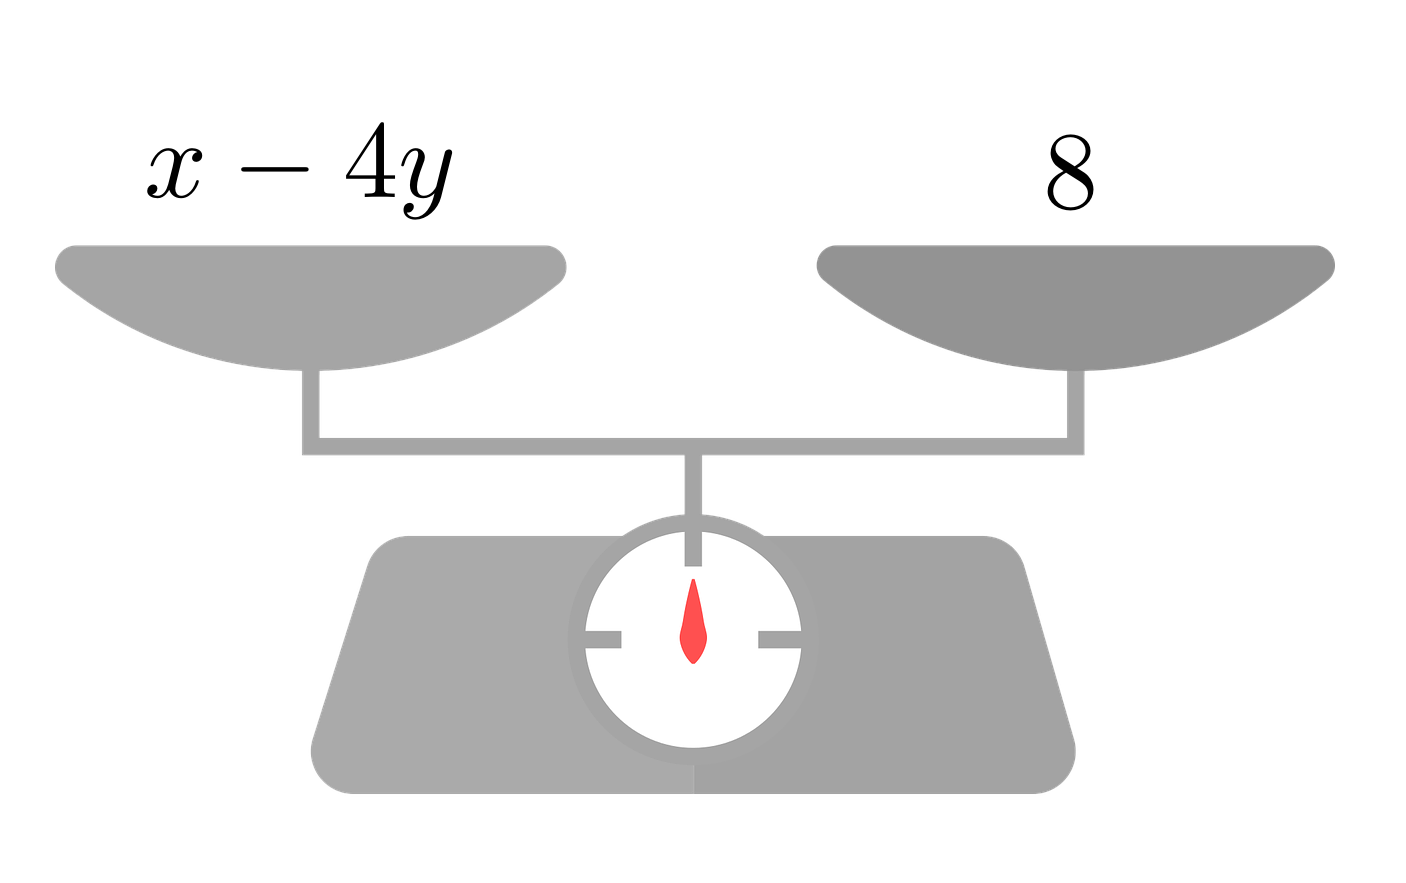
\includegraphics[width=6cm]{images/waage_x-4y=8.png}
		\end{minipage}
		\hfill
		\begin{minipage}{0.45\linewidth}
			\centering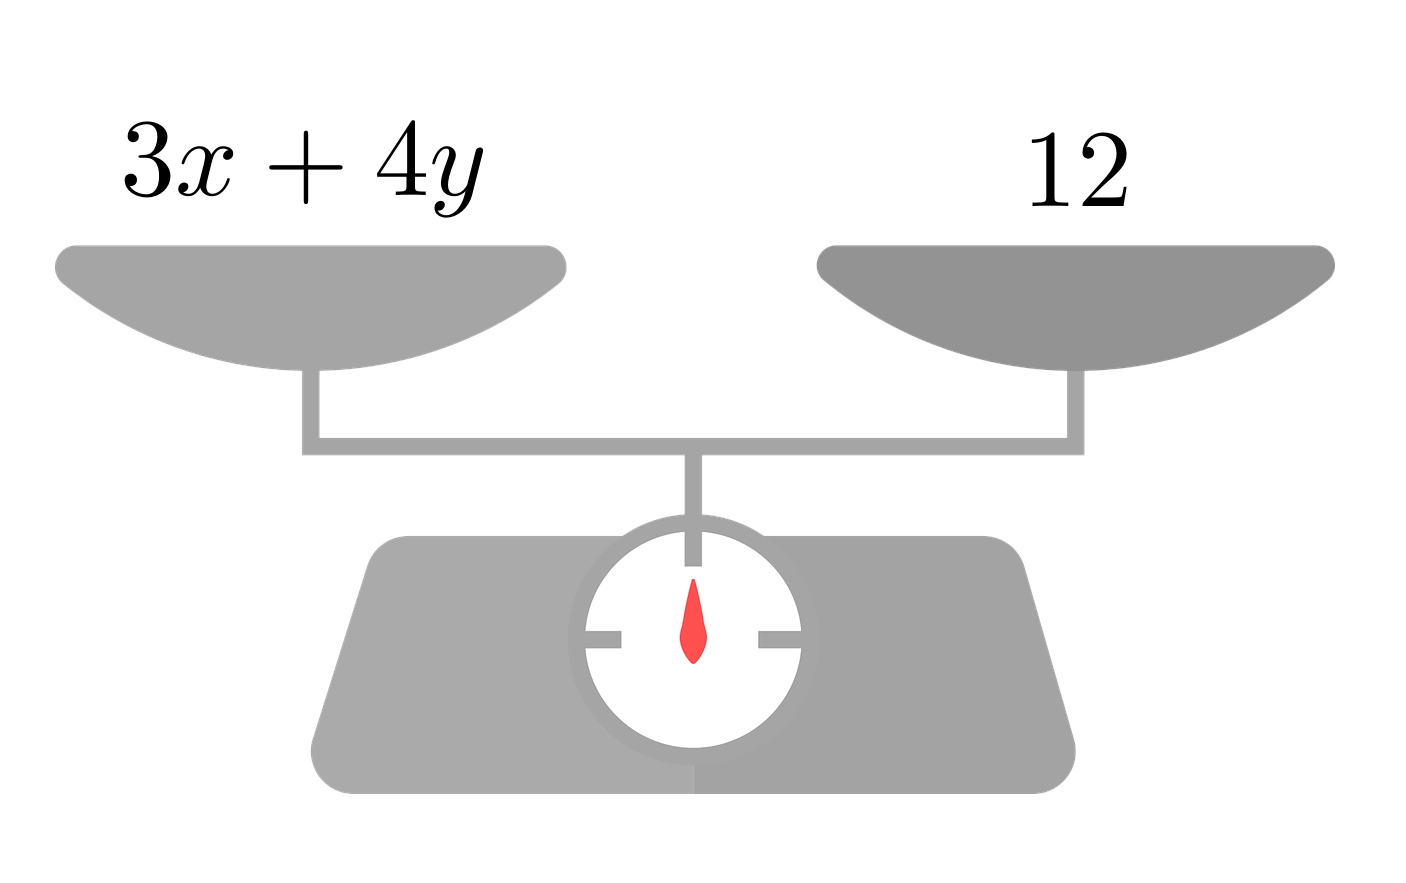
\includegraphics[width=6cm]{images/waage_3x+4y=12.png}
		\end{minipage}
		Legt man nun die Gegenstände der linken Waagschale und die Gegenstände der rechten Waagschale jeweils zusammen, so ergibt sich wieder ein Gleichgewicht.
		\begin{figure}[H]
			\centering
			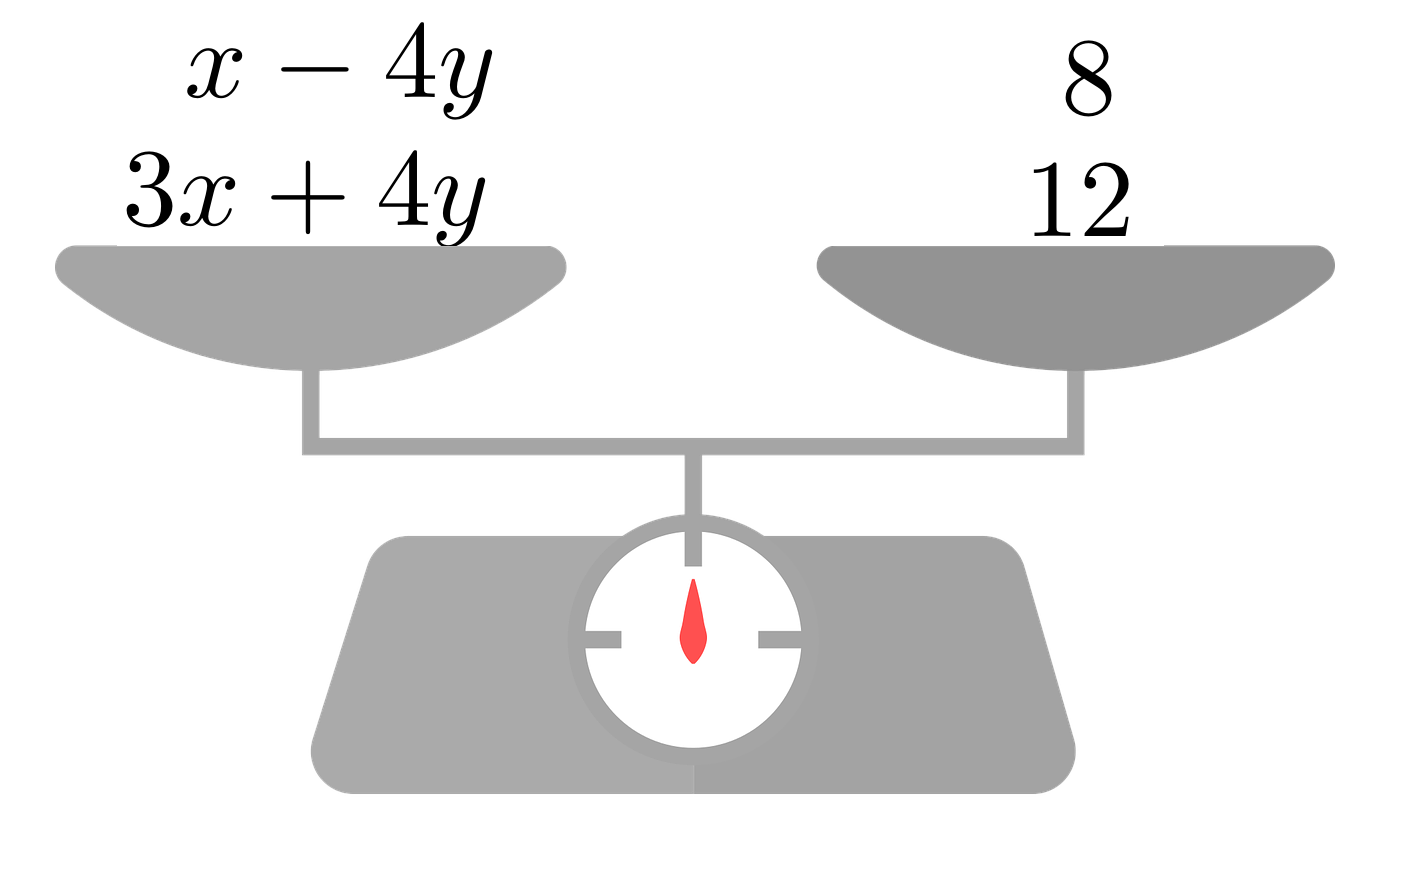
\includegraphics[width=6cm]{images/waage_beide.png}
		\end{figure}
		Die beiden Summen sind also wieder gleich gross:
		\begin{alignat*}{2}
			\text{I}:&\quad\phantom{x-4y+3}x-4y&&=8\\
			\text{II}:&\quad\phantom{x-4y+}3x+4y&&=12\\
			\cline{1-4}
			\text{I + II}: &\quad x-4y+3x+4y&&=8+12\\
			&\quad\phantom{x-4y+3x+}4x&&=20\\
			&\quad\phantom{x-4y+3x+4}x&&=5
		\end{alignat*}
		Wir bekommen also $x=5$.\\
		Setzt man diesen Wert 5 für $x$ in Gleichung I ein, so erhält man:
		\begin{align*}
			5-4y&=8\\
			y&=-\frac{3}{4}
		\end{align*}
		Die Lösung des Linearen Gleichungssystems lautet also:  $\underline{\underline{(5,-\frac{3}{4})}}$
	\end{beispiel}
	Damit man durch Addition der beiden Gleichungen eine Gleichung erhält, in der eine der beiden Variablen nicht mehr vorkommt, müssen die Koeffizienten dieser Variable in beiden Gleichungen den gleichen Betrag, aber unterschiedliche Vorzeichen besitzen (im Beispiel oben $-4y$ und $+4y$).\\
	Falls dies nicht der Fall ist, so muss man zuerst eine oder beide Gleichungen durch beidseitiges Multiplizieren mit geeigneten Zahlen umformen.
	\begin{beispiel}
		Lasst uns ein weiteres Gleichungssystem betrachten.
		\[\systeme{5x+6y=10,3x-2y=-22}\hspace*{12cm}\]
		Man kann hier das gleiche Verfahren anwenden, wenn man das Gleichungssystem vorher entsprechend \flqq präpariert\frqq: Wir multiplizieren die zweite Gleichung mit $3$, um auf $-6y$ zu kommen (entgegengesetzt gleich viele $y$ wie in der ersten Gleichung) und addieren diese mit $3$ multiplizierte Gleichung zur ersten Gleichung:\vspace*{5pt}\newline\karos{5.5}
	\end{beispiel}
	\begin{beispiel}
		\[\systeme{2x+5y=7, 3x+3y=\frac{3}{2}}\hspace*{12cm}\]
		\karos{9}
	\end{beispiel}
	\begin{algo}[Additionsverfahren]
		\begin{enumerate}[label=\Roman*)]
			\item Man bringt die beiden Gleichungen des Gleichungssystems (falls nötig) in die Standardform $ax+by=c$.
			\item Man eliminiert eine der beiden Variablen, indem man gegebenenfalls die beiden Gleichungen mit geeigneten Zahlen multipliziert und dann zueinander addiert bzw. voneinander subtrahiert.
			\item Man löst die dabei entstandene Gleichung in einer Unbekannten.
			\item Man bestimmt durch Einsetzen auch die zweite Unbekannte.
		\end{enumerate}
	\end{algo}
	\begin{aufgabe}
		blablabla
		\vspace{6cm}
	\end{aufgabe}
	\newpage

\section{Weitere Gleichungssysteme}
	Der Begriff des Gleichungssystems ist ein sehr allgemeiner. Wir schauen uns in diesem Abschnitt zunächst ein Beispiel eines nicht-linearen Gleichungssystems an. Danach arbeiten wir mit linearen Gleichungssystemen mit Parametern.
\subsection{Lineare Gleichungssysteme mit Parametern}
	Kommen neben den Lösungsvariablen noch weitere Variablen vor, so nennt man diese Parameter. Wenn nichts anderes geschrieben ist, werden die Lösungsvariablen mit $x$,$y$, ($z$) bezeichnet; wohin gegeb die Parameter häufig mit $a$, $b$ usw. bezeichnet werden.\vspace{5mm}

	In den allermeisten Fällen eignet sich das Additionsverfahren am Besten zur Lösung.
	\begin{beispiel}
		\begin{align*}
			ax + y &= b\\
			bx - y &= c
		\end{align*}
		\vspace{3cm}
	\end{beispiel}
	\begin{beispiel}[Beispiel (GZP 2015)]
		\begin{align*}
			a x + by &= 2\\
			bx + ay &= -2
		\end{align*}
		\vspace{3cm}
	\end{beispiel}
	\begin{aufgabe}
		Blablabla
		\vspace{4cm}
	\end{aufgabe}
	\newpage

\subsection{Nicht-lineare Gleichungssysteme}
	Wir betrachten die zwei Gleichungssysteme:\\
	\begin{minipage}{0.45\linewidth}
		\begin{equation}
			\label{eq:linSys}
			\systeme{\frac{1}{4}x+y=7, x+y=10}\hspace{1.5cm}
		\end{equation}
	\end{minipage}
	\hfill
	\begin{minipage}{0.45\linewidth}
		\begin{equation}
			\label{eq:nonlinSys}
			\systeme{\frac{1}{4}x\cdot y=12, y=\frac{3}{4}x}
		\end{equation}
	\end{minipage}
	Das System \ref{eq:linSys} ist ein \emph{lineares Gleichungssystem}. In den Gleichungen werden die Unbekannten nur mit Zahlen multipliziert. Gleichungssystem \ref{eq:nonlinSys} ist nichtlinear, denn hier werden die zwei Unbekannten miteinander mulitpliziert.
	\begin{definition}[LGS: Lineares Gleichungssystem]
		Ein \emph{lineares Gleichungssystem} besteht ausschliesslich aus linearen Gleichungen, d.h. die Unbekannten werden nur mit Zahlen multipliziert.
	\end{definition}
	\begin{aufgabe}
		Welches der folgenden Gleichungssysteme ist linear, welches nichtlinear?
		\begin{enumerate}[label=\alph*)]\begin{multicols}{2}
				\item \systeme{3x-2y=(-1)^2,x+y=4}
				\item \systeme{(y-1)^2+x =7 x - y+y^2, \frac{x}{2}+\frac{y}{4}= -1}
		\end{multicols}\end{enumerate}
	\end{aufgabe}

\subsection{Auf lineare zurückführbare Gleichungen}
	Einige Gleichungen lassen sich durch Ausmultiplizieren auf lineare Gleichungen zurück-führen. Andere nichtlineare Gleichungen lassen sich durch eine geeignete Substitution (d.h. Ersetzen eines Ausdrucks durch einen neuen) auf lineare Gleichungen zurückführen. So können sie mit den bekannten Mitteln aufgelöst werden. Anschliessend muss die Substitution rückgängig gemacht werden.

	Wir betrachten zu beiden Vorgehen je zwei Beispiele:
\subsection*{Lösen durch Multiplikation}
	\begin{beispiel}
		\begin{align*}
			\frac{2x+5}{8x+y}&=\frac{1}{2}\\
			\frac{5x-2y}{5x+2y}&=\frac{19}{11}
		\end{align*}\vspace{3cm}
		\begin{align*}
			\frac{1}{x}+\frac{1}{y}&=\frac{1}{xy}\\
			\frac{1}{x}-\frac{1}{y}&=\frac{2}{xy}
		\end{align*}\vspace{4cm}
	\end{beispiel}
	\begin{aufgabe}
		Blablabla
		\vspace{2cm}
	\end{aufgabe}
\subsection*{Substitution}
	\begin{align*}
		\frac{1}{x}+\frac{1}{y}&=7\\
		\frac{1}{x}-\frac{1}{y}&=1
	\end{align*}\vspace{3cm}
	\begin{align*}
		\frac{5}{x+y}-\frac{3}{x-y}&=4\\
		\frac{2}{x+y}+\frac{6}{x-y}&=4
	\end{align*}\vspace{5cm}
	\begin{aufgabe}
		Blablabla
		\vspace{2cm}
	\end{aufgabe}
	\newpage

\section{Das Gauss-Verfahren}

	\newpage



\section{Textaufgaben}


\subsection{Mischaufgaben}
	Zum Abschluss des Kapitels zu Linearen Gleichungssystemen betrachten wir Textaufgaben.\\
	Im Skript wollen wir einen speziellen Aufgabentyp von Textaufgaben etwas genauer betrachten. Bei Mischaufgaben werden zwei Objekte (z.B. Flüssigkeiten, Metalle...)  mit unterschiedlicher Eigenschaft (z.B. Salzgehalt, Goldgehalt, Alkoholgehalt, Dichte...) miteinander vermischt.
	\\
	Wir betrachten das Vorgehen zur Lösung an einem typischen Beispiel.\\
	Die erste Aufgabe lässt sich noch direkt berechnen.
	\begin{beispiel}
		2 Liter 70\%-ige Salzlösung (Salzgehalt 70\%) werden mit 5 Liter Wasser verdünnt. Wie gross ist nun der Salzgehalt?\\
		\textbf{Antwort: } In der Mischung sind $0.7\cdot 2$ Liter Salz, verteilt auf 7 Liter.
		Der Salzanteil beträgt also $\frac{0.7\cdot 2}{7}=0.2=20\%$
	\end{beispiel}
	\noindent
	In der nächsten Aufgabe brauchen wir eine Variable:
	\begin{beispiel}
		Mit wieviel Liter Wasser müssen 3 Liter 80\%-ige Salzlösung verdünnt werden, damit eine 30\%-ige Salzlösung entsteht?\\
		\textbf{Antwort: } Die Menge Wasser bezeichnen wir mit $x$. In der Mischung sind somit $0.8\cdot 3$ Liter Salz, verteilt auf $3+x$ Liter. Somit muss gelten:
		\begin{align*}
			\dfrac{0.8\cdot 3}{3+x}&=0.3 \\
			\Rightarrow& x=5
		\end{align*}
	\end{beispiel}
	\noindent
	Im nächsten Beispiel empfiehlt sich die Nutzung von zwei Variablen:
	\begin{beispiel}
		Wie müssen eine 30\%-ige und 80\%-ige Salzlösung gemischt werden, um 5 Liter einer 45\%-igen Salzlösung zu erhalten?\\
		\textbf{Antwort: } In der Mischung von $x$ Litern 30\%-ige und $y$ Litern 80\%-ige Salzlösung sind $0.3x+0.8y$ Liter Salz. In den 5 Litern 45\%ige Salzlösung müssen $0.45\cdot 5$ Liter Salz enthalten sein. Zusammen mit der Bedingung, dass $x+y=5$ erhalten wir ein LGS:
		\begin{center}
			\systeme{x+y=5, 0.3x+0.8y=0.45\cdot 5}
		\end{center}
		Die Lösung lautet: $x=3.5$, $y=1.5$. Also müssen 3.5 Litern der 30\%-igen Salzlösung mit 1.5 Litern der 80\%-igen Salzlösung gemischt werden, um 5 Liter einer 45\%-igen Salzlösung zu erhalten.\\
		\emph{(Bemerkung: Man könnte auch nur eine Variable $x$ verwenden und die Menge der zweiten Flüssigkeit als $5-x$ benutzen. )}
	\end{beispiel}
	\noindent Schauen wir uns die letzte Aufgabe tabellarisch nochmals an:\\
	\begin{table}[h]
		\centering
		\begin{tabular}{ c|c|c|c}

			& 30\%-ige Salzlösung & 80\%-ige Salzlösung & Mischung  \\ \hline
			Menge (V)&	$V_1=x$ & $V_2=y$ & \color{lightgray} $V_3=5$\\
			Gehalt (p)& $p_1=0.3$ & $p_2=0.8$ &\color{lightgray} $ p_3=0.45$ \\
			Salzmenge & $p_1\cdot V_1=0.3x$ & $p_2\cdot V_2=0.8y$ & $p_3\cdot V_3=0.45\cdot 5$
		\end{tabular}
		\caption*{Typische Mischaufgabe}
		\label{tab:TypischeMischaufgabe}
	\end{table}
	\begin{figure}[H]
		\centering
		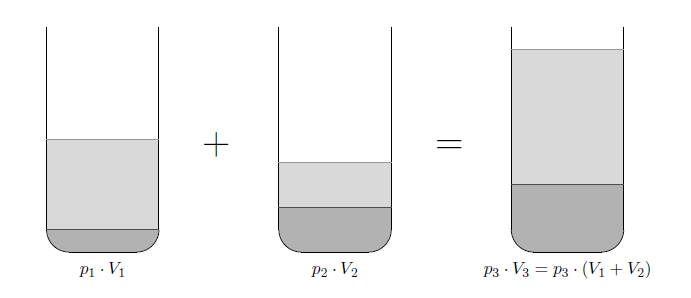
\includegraphics[width=0.8\textwidth]{images/mischaufg.png}
		\label{fig:mischaufg}
	\end{figure}
	Die Grafik veranschaulicht die Salzmenge. Die Volumen $V_1$, $V_2$ und $V_3$ stehen für die Mengen der einzelnen Salzlösungen. $p_1$, $p_2$ und $p_3$ stehen für den jeweiligen Gehalt. So hat beispielsweise in der ersten Flüssigkeit $ p_1\cdot V_1$ (bzw. $0.3x$) Salz.\\
	Klar ist, dass beim Mischen keine Flüssigkeit verloren geht, also $V_1+V_2=V_3$.\\
	Dann nützen wir aus (siehe Tabelle), dass die Salzmenge sich vor und nach dem Mischen nicht ändert (sie addieren sich nur):\vspace{-0.5cm}
	\begin{align*}
		p_1\cdot V_1 + p_2\cdot V_2&=p_3\cdot V_3\\
		0.3x+0.8y&=0.45\cdot 5.
	\end{align*}
	Das ergab uns die zweite Gleichung. \\
	Wir könnten auch den Gehalt der dritten Flüssigkeit $p_3$ durch die andern Grössen ausdrücken.
	\begin{align*}
		p_1\cdot V_1 + p_2\cdot V_2&=p_3\cdot V_3\\
		\Rightarrow p_3&=\dfrac{p_1\cdot V_1 + p_2\cdot V_2}{V_3}\\
		p_3&=\dfrac{p_1\cdot V_1 + p_2\cdot V_2}{V_1+V_2}\\
		0.45&=\frac{0.3x+0.8y}{x+y}
	\end{align*}
	Statt die zweite Gleichung $0.3x+0.8y=0.45\cdot 5$ könnte man also auch $0.45=\dfrac{0.3x+0.8y}{x+y}$ im LGS benutzen.\\
	Das obige Prinzip funktioniert für alle Mischaufgaben.
	\begin{framed}
		\begin{itemize}
			\item Schreibe alle relevanten Grössen tabellarisch auf.
			\item Verbinde die Grössen mit Gleichungen. D.h. schreibe vorkommende Grössen auf zwei unterschiedliche Arten auf.
		\end{itemize}
	\end{framed}
	\newpage


\subsection*{History}
\begin{table}[H]
	\centering
	\begin{tabular}{|p{13mm}|p{20mm}|p{30mm}|p{70mm}|}\hline
		%\multicolumn{4}{|l|}{History}\\\hline
		Version & Datum & Person & Bemerkung \\\hline
		$0.1$ & 02.08.2024 & Jonas Guler & Kapitel von Hs übernommen \\\hline
		$0.2$ & ToDo & Jonas Guler & Überarbeitung \\\hline
	\end{tabular}
\end{table}

\newpage
\appendix
\section*{Einführung}
	Lineare Gleichungssysteme wurden schon vor sehr langer Zeit betrachtet. Mit dem Aufstieg von Königreichen in Mesopotamien, Ägypten, Indien und China fingen die Menschen an, das hervorzubringen was wir Kultur nennen. Dazu gehört auch die Mathematik.\\
	Schon damals wurden die Kenntnisse, welche sie entwickelten, in Lehrbüchern aufbewahrt. In ihnen wurde gezeigt, wie Probleme durch Rechnen gelöst werden können. Allerdings gab es dazu noch keine Theorie, man lernte einzig an Beispielen (wie bei uns häufig noch in der Primarschule).\\
	Wir betrachten zum Einstieg einige solche historische Aufgaben:
	\begin{center}
		\begin{framed}
			Historische Aufgabe 1 (Mesopotamien, ca. 2000 v. Chr):\\
			\glqq Ein Viertel der Breite zur Länge addiert ergibt 7 Handbreiten, Länge und Breite addiert macht 10 Handbreiten\grqq.
		\end{framed}
	\end{center}
	Das Problem also ist, dass man Breite und Länge - vielleicht von einem rechteckigen Stück Tuch - nicht kennt. Andererseits wissen wir zwei Dinge:
	\begin{enumerate}[label=\alph*)]
		\item Ein Viertel der Breite, zur Länge addiert, gibt $7$ Handbreiten
		\item Länge und Breite zusammengezählt machen $10$ Handbreiten aus
	\end{enumerate}
	Wir eilen der Zeit um gut dreieinhalb Jahrtausende voraus, wenn wir die unbekannte Breite mit $x$, die unbekannte Länge mit $y$ bezeichnen und die uns vertrauten Zeichen $+$ und $=$ verwenden. Der französische Mathematiker und Philosoph René Descartes $\left(1596-1650\right)$ war übrigens der erste, der unbekannte Grössen mit den Buchstaben $x,y,z$ bezeichnete. Heute drücken wir die obigen Aussagen so aus:
	\begin{align*}
		\frac{1}{4}\cdot x + y &= 7 \\
		x + y &= 10
	\end{align*}

	\begin{center}
		\begin{framed}
			Historische Aufgabe 2 ("`aus Papyrus Moskau, Ägypten, ca. 2000 v. Chr.):\\
			"`Berechne die Länge und Breite eines Rechteckes
			der Fläche 12, wenn die Breite 3/4 der Länge ist."'
		\end{framed}
	\end{center}
	Wir bezeichnen mit x die Länge, mit y die Breite des Rechteckes. Wir
	erhalten wieder zwei Gleichungen:
	\begin{center}
		(i) $x\cdot y=12$\\
		(ii) $y = \frac{3}{4}x$
	\end{center}
	\begin{center}
		\begin{framed}
			Historische Aufgabe 3 (aus Lehrbuch von Diophant 250 n. Chr., Griechenland):\\
			"`Jemand drückt 100 auf zwei verschiedene Arten aus und zwar so, dass ein Summand der ersten Summe das Doppelte eines Summanden der zweiten Summe ist und dass der andere Summand der zweiten Summe das Dreifache des anderen Summanden der ersten Summe ist. Wie heissen die Zahlen?"'
		\end{framed}
	\end{center}
	\begin{center}
		\begin{framed}
			Historische Aufgabe 4 ("`Problem der 100 Vögel"', China, 475 n. Chr):\\
			"`Ein Hahn kostet 5 sapek, eine Henne 3 sapek und drei Küken 1 sapek. Wenn wir nun für 100 sapek 100 dieser Tiere einkaufen: Wie viele sind es dann von jeder Sorte?"'
		\end{framed}
	\end{center}
	Obige Aufgabe ist ein sehr berühmtes Problem. Das sich in andern Varianten bei den Indern , Arabern, in Byzanz und schliesslich fast bei allen Mathematikern in Europa wiederfindet.
	\begin{center}
		\begin{framed}
			Historische Aufgabe 5 (aus "`Rechenbuch auff Linien und Ziphren"', Adam Ries (1492-1559)):\\

			"`Item, einer hat 100 Gulden. dafür will er 100 Haupt Vihes kauffen / nemlich / Ochsen / Schwein / Kälber / und Geissen / Kost ein Ochs 4 Gulden. ein Schwein anderthalb Gulden. ein Kalb
			einen halben Gulden. und ein Geiss ein ort [\textit{d.h. ein Viertel}] von einem Gulden. wie viel sol er jeglicher haben für die 100 Gulden?"'
		\end{framed}
	\end{center}

	Als letztes Beispiel betrachten wir eine Aufgabe des Rechenmeisters Michael Stifel. Er nennt diese ein "`schönes Beispiel"'. Wohl im Gegensatz zu den gewöhnlichen, eher trostlosen Übungsaufgaben.
	\begin{center}
		\begin{framed}
			Historische Aufgabe 6 (von Michael Stifel (1487-1567)):\\

			"`Drei Reisende finden, während sie zusammen so dahingehen, einen Ranzen mit 73 Gulden. Sie stellen fest, dass diese 73 Gulden zusammen mit der Barschaft der ersten beiden das Doppelte dessen sind, was der erste und dritte und der zweite und dritte gemeinsam bei sich haben. Diese 73 Gulden ergeben aber auch mit dem Besitz des ersten und dritten das Dreifache dessen, was der zweite und dritte und der erste und zweite mit sich führen. Und schliesslich ergeben diese 73 Gulden zusammen mit der Barschaft des zweiten und
			dritten das Vierfache dessen, was der erste und zweite und der erste
			und dritte zusammen bei sich tragen. Wie viele Gulden besitzt jeder?"'
		\end{framed}
	\end{center}
	\begin{aufgabe}
		Gib für die historischen Aufgaben 3 bis 6 jeweils die Unbekannten an und formuliere die Gleichungen, die für diese Unbekannten gelten.
	\end{aufgabe}

	\begin{definition}[Gleichungssystem]
		Immer, wenn man für eine Anzahl Unbekannte eine Anzahl Gleichungen hat, spricht man von einem \emph{Gleichugnssystem}.
	\end{definition}
	\newpage

\section*{Was sind Lösungen eine Gleichungssystems?}
	In einem Gleichungssystem geht es darum, die Unbekannten so zu bestimmen, dass mit dieser Wahl alle Gleichungen erfüllt werden. Nehmen wir das System der ersten historischen Aufgabe:
	\begin{equation}
		\label{eq:firstSys}
		\systeme{\frac{1}{4}\cdot x+y=7, x+y=10}
	\end{equation}
	Wählen wir 2 für x und 6.5 für y wird die erste Gleichung erfüllt, die zweite jedoch nicht. Umgekehrt erfüllen die Zahlen 3.8 für x und 6.2 für y zwar die zweite, nicht aber die erste Gleichung.\\
	Wenn wir hingegen für x die Zahl 4 und für y die Zahl 6 wählen, so sind \emph{beide} Gleichungen erfült:
	\begin{align*}
		\frac{1}{4}\cdot 4 +6 &= 7\\
		4+6&=10
	\end{align*}
	Man drückt dies so aus:
	\begin{center}\glqq Das Zahlenpaar (4, 6) ist eine Lösung des Systems \ref{eq:firstSys}\grqq\end{center}
	\begin{definition}[Lösung eines Gleichungssystems]
		Eine Lösung eines Gleichungssystems ist eine Zuordnung an die Unbekannten, so dass alle Gleichungen des Systems erfüllt werden.
	\end{definition}
	Werden die Unbekannten mit \emph{Buchstaben} bezeichnet, so gilt die lexikalische Ordnung. Die erste Zahl steht für den Buchstaben, der im Alphabet zuerst kommt.\\
	Falls wir \emph{indizierte Unbekannte} (z.B. $x_1, x_2, x_3...$) verwenden, so ist die Reihenfolge ebenfalls klar.
	Betrachten wir zum Beispiel das Gleichungssystem:
	\begin{equation*}
		\systeme{x_1+x_2+x_3=100, 5x_1+3x_2+\frac{1}{3}x_3=100}
	\end{equation*}
	Dann ist die Aussage "`Das Zahlentripel $\big(\frac{20}{3},\frac{40}{3},80\big)$ ist Lösung dieses Gleichungssystemes"' unmissverständlich. Die erste der drei umklammerten Zahlen entspricht der ersten Unbekannten $x_1$, die zweite Unbekannten $x_2$, und so weiter. Mit solchen indizierten Unbekannten kann eine beliebig grosse Anzahl von Unbekannten erfasst werden. Dies ist bei modernen Anwendungen mit Tausenden Unbekannten natürlich unabdingbar.
	\begin{aufgabe}
		Welche der Zahlentripel (0,0,0), (4,3,5), (4,5,3), (5,4,3), (-2,5,-12), (-2, -12,5), (2,12,5), (2,12,-9) sind Lösungen der Gleichung:
		\begin{align*}
			5x_1-2x_2=2x_3+4
		\end{align*}
	\end{aufgabe}
	\begin{aufgabe}
		Welche der Tripel (2.15,-2.65.0), (1.65,-1.15,1), (1.4,0.4,1.5), (2.4,-3.4,-0.5) sind Lösungen des Gleichungssystems:
		\begin{equation*}
			\systeme{3.1x+2.1y-1.6z-1.1=0,3.9x+2.9y-2.4z-0.7=0}
		\end{equation*}
	\end{aufgabe}
	\begin{aufgabe}
		Betrachte die Gleichung $x+y+z-2=0$ und bestimme sämtliche Lösungen, die nur aus nichtnegativen ganzen Zahlen bestehen.
	\end{aufgabe}
	\newpage


\section*{Gleichungssysteme geometrisch betrachtet}
	Wir betrachten ein 2x2 lineares Gleichungssystem.
	\begin{equation*}
		\systeme{3x-6y=18, 6x+4y=12}
	\end{equation*}
	Lösen wir beide Gleichungen nach $y$ auf so erhalten wir:
	\begin{equation*}
		\systeme{y=\frac{1}{2}x-3, y=-\frac{3}{2}x+3}
	\end{equation*}
	Die Lösungen der ersten Gleichung werden durch die Punkte einer Geraden $g$ dargestellt. Diejenigen der zweiten Gleichung entsprechen einer andern Geraden $h$.
	\begin{figure}[H]
		\centering
		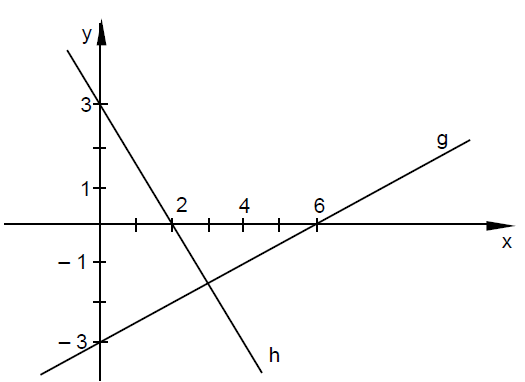
\includegraphics[width=0.5\textwidth]{images/geomlgs.png}
	\end{figure}
	Im vorliegenden Fall hat das Gleichungssystem genau eine Lösung. Nämlich der Schnittpunkt der beiden Lösungsgeraden ($3,-1.5$). Wie sehen die andern Fälle eines linearen Gleichungssystems mit zwei Unbekannten aus?\\
	Wir haben gesehen, dass ein lineares Gleichungssystem keine, eine oder unendlich viele Lösungen haben kann. Entsprechend ergeben sich die folgenden drei Fälle:
	\begin{figure}[H]
		\centering
		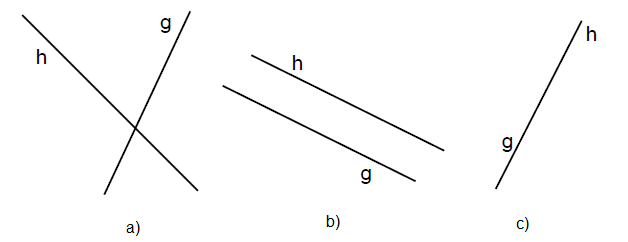
\includegraphics[width=0.6\textwidth]{images/lgsfaelle.png}
	\end{figure}
	\begin{enumerate}[label=\alph*)]
		\item Im ersten Fall schneiden sich wie oben die Geraden. Das entsprechende Gleichungssystem ist \emph{eindeutig} lösbar.
		\item Im zweiten Fall sind die Geraden parallel und veschieden. Das Gleichungssystem ist \emph{unlösbar}.
		\item Im letzten Fall fallen die Geraden gerade zusammen. Das Gleichungssystem hat \emph{unendlich viele} Lösungen.
	\end{enumerate}
	\begin{aufgabe}
		Löse jeweils mithilfe Graphen (auf einem separaten Blatt):
		\begin{figure}[H]
			\centering
			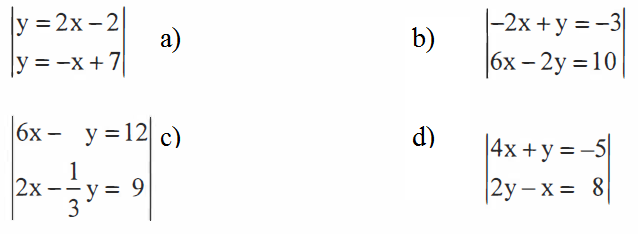
\includegraphics[width=8cm]{images/lgsg.PNG}
		\end{figure}
	\end{aufgabe}
	\begin{aufgabe}[Unterwegs mit der Bahn]
		Ein Interregio startet um 6 Uhr in Arbeitsstedt und fährt dann mit einer Durchschnittsgeschwindigkeit von 120 km pro Stunde über Freital nach Schlafhausen. Ein Vorortszug startet um 6 Uhr in Freital auf einem Gleis, das neben dem des Interregio verläuft. Sein Ziel ist ebenfalls Schlafhausen, seine Durchschnittsgeschwindigkeit 100 km pro Stunde. Arbeitsstedt und Freital sind 10 km voneinander entfernt, Arbeitsstedt und Schlafhausen 500 km.\\
		Versuche möglichst einfach herauszufinden, wann der Interregio den Vorortszug einholt. Du darfst hierbei auch sinnvoll probieren. Wo befinden sich die Züge dann?
	\end{aufgabe}
	\begin{aufgabe}[Zaubertrick]
		\begin{figure}[H]
			\centering
			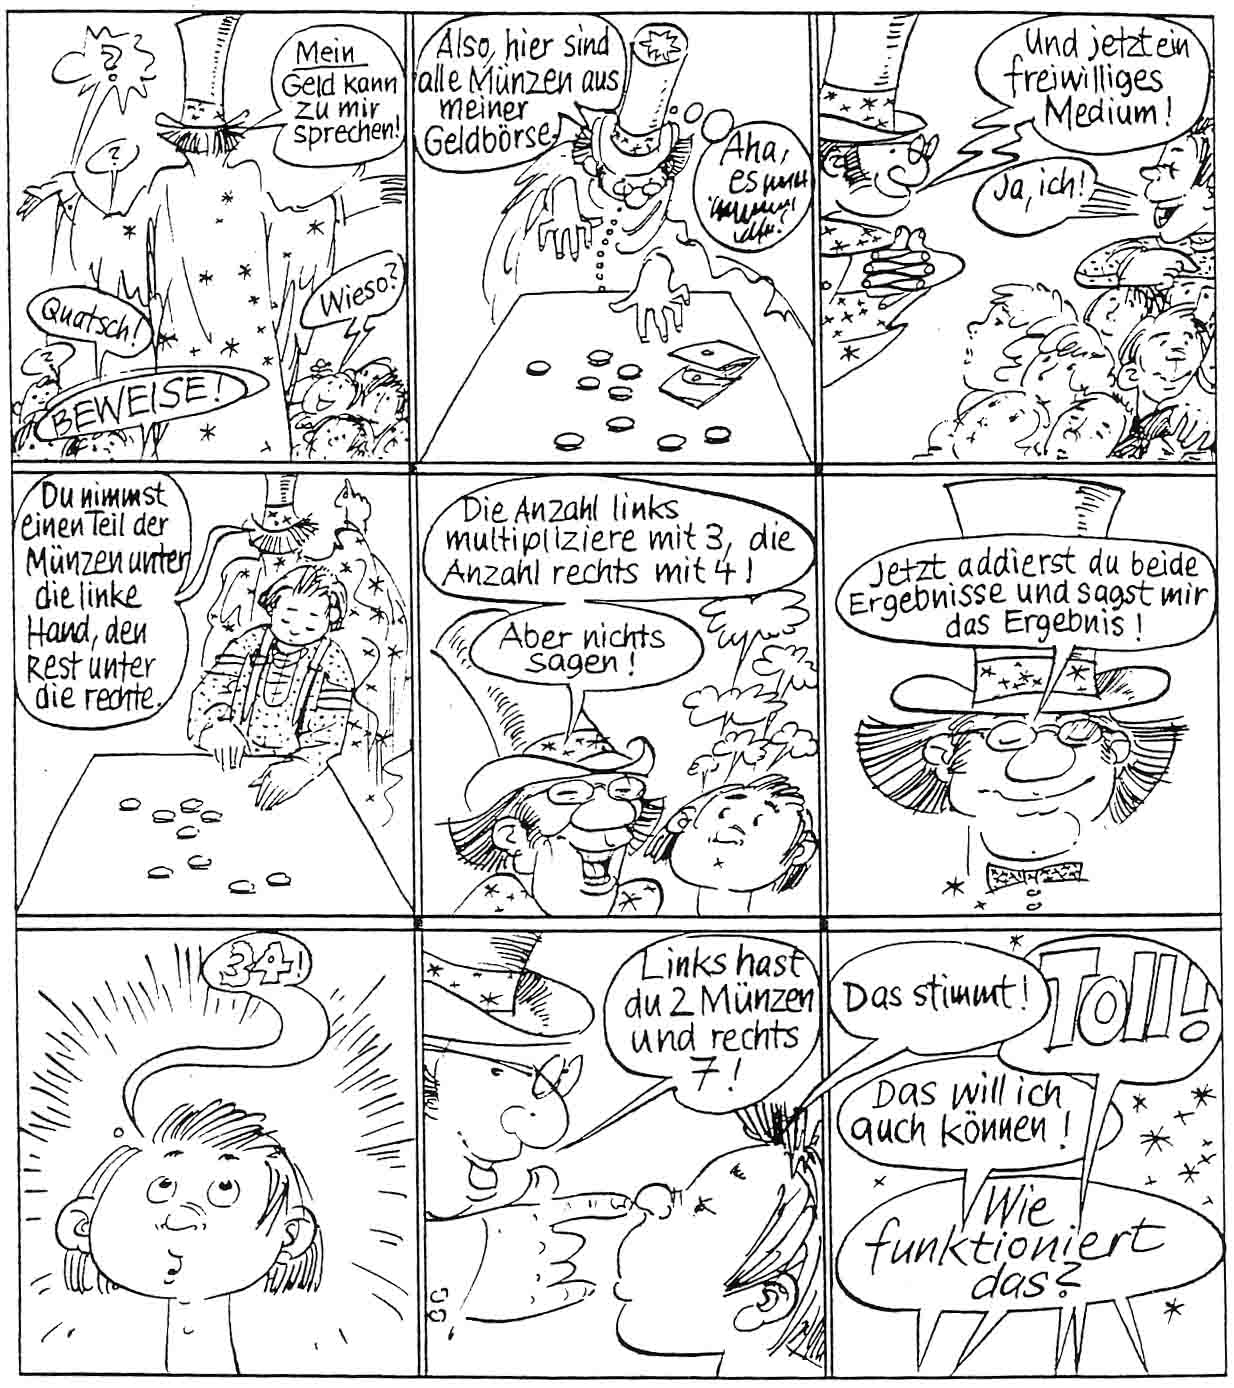
\includegraphics[width=7cm]{images/zaubertrick.png}
		\end{figure}
		Versuche herauszufinden, wie der Zaubertrick des Magiers funktioniert.
	\end{aufgabe}
	\newpage


\subsection*{Das Gleichsetzungsverfahren}
	Dieses Verfahren kennen wir von der Berechnung des Schnittpunkts zweier Geraden (siehe wieder \flqq lineare Funktionen\frqq).
	Wir betrachten nochmals das Beispiel aus der geometrsichen Betrachtung.
	\begin{align*}
		\systeme{3x-6y=18, 6x+4y=12}
	\end{align*}
	Durch geeignetes algebraischen Umformen können beiden Gleichungen nach derselben Variablen (entweder nach $y$ oder nach $x$) aufgelöst werden.So erhalten wir die Gleichungen:
	\begin{align*}
		\systeme{y=\frac{1}{2}x-3, y=-\frac{3}{2}x+3}
	\end{align*}
	Nun haben wir uns überlegt, dass die Lösungen der ersten Gleichungen auf dem Graphen der Funktion $y=\frac{1}{2}x-3$ liegen. Umgekehrt liegen die Lösungen der zweiten Gleichung auf dem Graphen der Funktion $y=-\frac{3}{2}x+3$.\\
	A, B, S und D sind Lösungen von $y=-\frac{3}{2}x+3$.
	C, S und E sind Lösungen von  $y=\frac{1}{2}x-3$ .
	\begin{figure}[H]
		\centering
		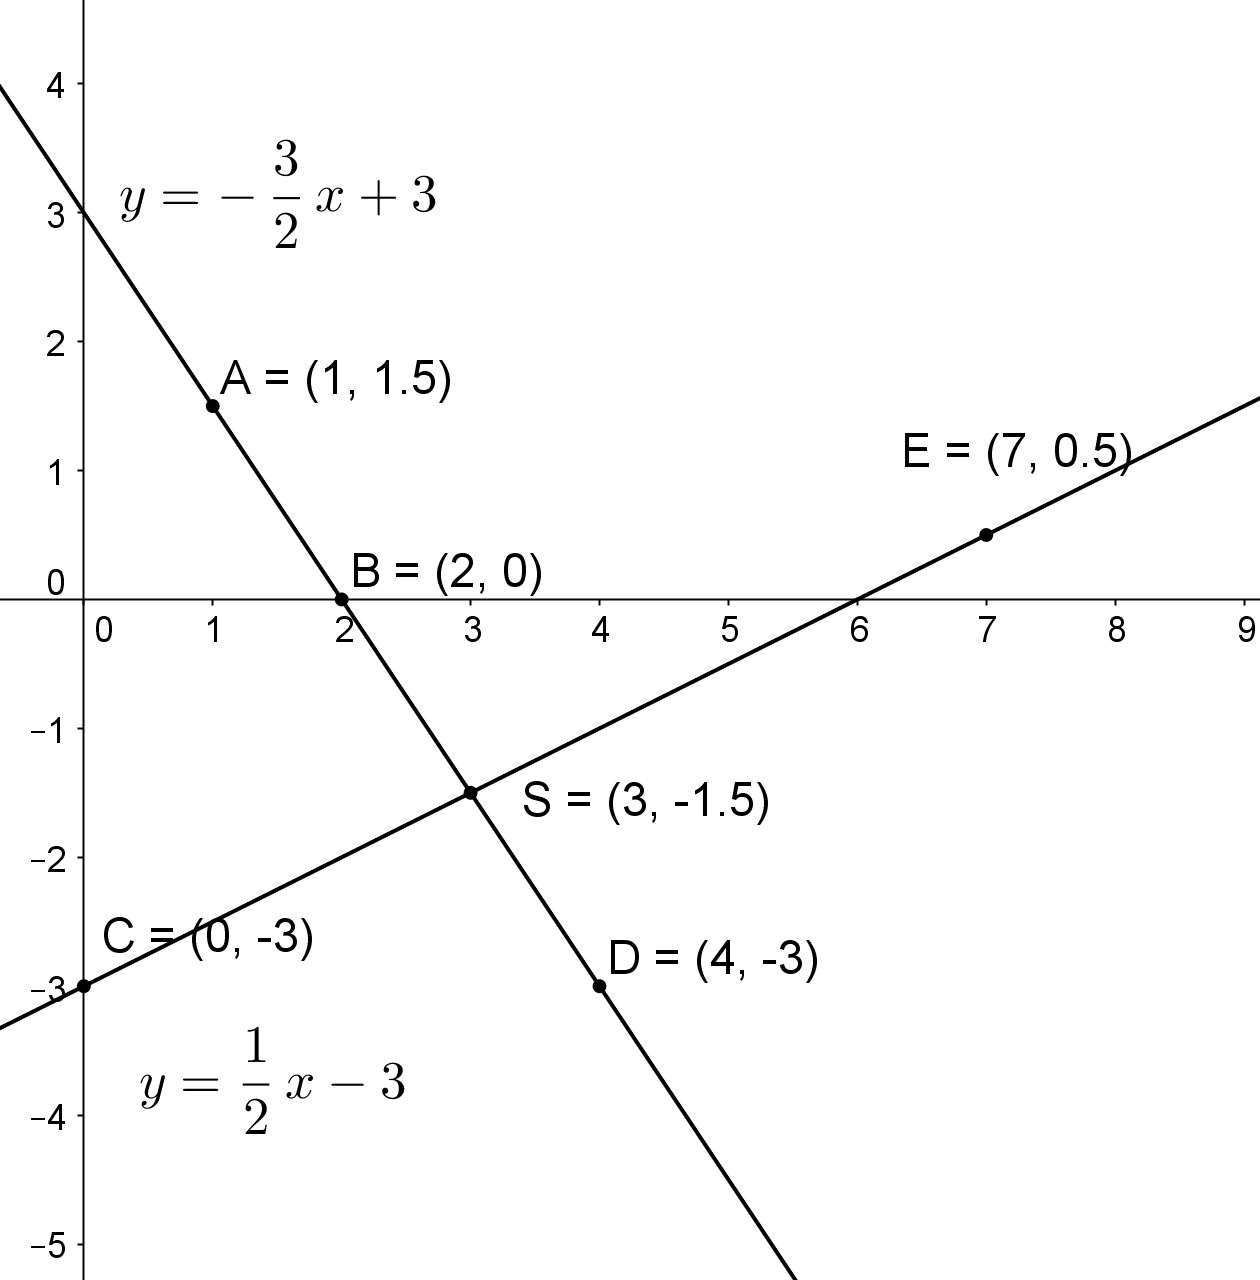
\includegraphics[width=8cm]{images/gleichsetz.png}
	\end{figure}
	Die gemeinsame Lösung der beiden Gleichungen ist gerade der Schnittpunkt $S$. \\ Diesen finden wir durch Gleichsetzen der beiden Gleichungen und Auflösen nach $x$. Anschliessend müssen wir mit Einsetzen in eine der beiden Gleichungen noch $y$ bestimmen.
	\begin{beispiel}
		In obigem Beispiel wurden die Gleichungen \systeme{3x-6y=18, 6x+4y=12} nach $y$ aufgelöst, das ergab \systeme{y=\frac{1}{2}x-3, y=-\frac{3}{2}x+3}.
		Nun müssen wir diese Gleichsetzen:
		\begin{align*}
			\frac{1}{2}x-3&=-\frac{3}{2}x+3\\
			2x&=6\\
			x&=3
		\end{align*}
		Nun müssen wir noch das zugehörige $y$ bestimmen:
		\begin{align*}
			y&=\frac{1}{2}x-3\\
			y&=\frac{1}{2}\cdot 3-3\\
			y&=-\frac{3}{2}
		\end{align*}
		Damit haben wir die Lösung des Gleichungssystems gefunden: $\underline{\underline{(3,-\frac{3}{2})}}$
	\end{beispiel}
	\newpage

\subsection*{Vertiefung Einsetzungsverfahren}
	\begin{aufgabe}
		Adaptiere den Lösungsvorgang mit zwei Gleichungen auf das untenstehende lineare Gleichungssystem mit 3 Gleichungen und 3 Unbekannten. Findest du die Lösungen?
		\begin{equation*}
			\systeme{3x-2y+5z=23, 4x+8y-2z=-6, 5x+2y+2z=14}
		\end{equation*}
	\end{aufgabe}
	In obiger Aufgabe haben wir gesehen, dass auch für ein System von linearen Gleichungen mit mehr als zwei Gleichungen/Unbekannten das Verfahren der Substitutions funktioniert.\\
	Man löst eine Gleichung nach einer Unbekannten auf und setzt das Ergebnis in die anderen Gleichungen ein. Hat man also zu Beginn beispielsweise 10 Gleichungen mit 10 Unbekannten, so hat man nach diesem Schritt ein System mit 9 Gleichungen und 9 Unbekannten. Man wiederholt den Schritt und kommt auf 8 Gleichungen mit 8 Unbekannten. Man macht dies weiter bis nur noch eine Gleichung mit einer Unbekannten übrig bleibt. Diese wir gelöst und eine Unbekannte ist somit bestimmt. Indem wir den ganzen Weg rückwärts gehen, können wir nun auch die andern Unbekannten sukzessive bestimmen.
	\begin{beispiel}
		Wir betrachten ein System mit 4 Gleichungen und 4 Unbekannten:
		\begin{equation*}
			\systeme{x_1+x_2-x_3+x_4=0, x_1-x_2-x_3-x_4=0, x_1+x_2+x_3-x_4=5, x_1-x_2+x_3+x_4=3}
		\end{equation*}
		Wählen wir zum Auflösen die 4. Gleichung und lösen sie nach $x_4$ auf, das ergibt $x_4=-x_1+x_2-x_3+3$. Wir setzen dies in die ersten drei Gleichungen ein und erhalten:
		\begin{equation*}
			\systeme{2x_2-2x_3+3=0, 2x_1-2x_2-3=0, 2x_1+2x_3-3=5}
		\end{equation*}
		Vereinfachen wir jede Gleichung indem wir die Zahlen auf die rechte Seite des Gleichheitszeichens schieben. Damit erhalten wir:
		\begin{equation*}
			\systeme{2x_2-2x_3=-3, 2x_1-2x_2=3, 2x_1+2x_3=8}
		\end{equation*}
		Also bleibt schonmal ein System mit 3 Gleichungen und 3 Unbekannten übrig. Wir lösen nun die 3. Gleichung nach $x_3$ auf: $x_3=-x_1+4$. Eingesetzt in die beiden anderen Gleichungen und Umformen ergibt:
		\begin{equation*}
			\systeme{2x_1+2x_2=5, 2x_1-2x_2=3}
		\end{equation*}
		Mit $x_2=x_1-1.5$ aus der zweiten Gleichung eingesetzt in die erste folgt: $4x_1=8$, also $x_1=2$. Mittels "`Rückwärtseinsetzen"' findet man nun sukzessive die übrigen Unbekannten:
		\begin{align*}
			x_1&=2\\
			x_2&=2-1.5=0.5\\
			x_3&=-2+4=2\\
			x_4&=-2+0.5-2+3=-0.5
		\end{align*}
		Wir sehen also, dass dieses Lösungsschema für beliebig grosse lineare Gleichungssysteme funktioniert und wir eine Lösung finden. Es ist auch leicht zu erkennen, dass je mehr Gleichungen im System sind, desto aufwendiger ist das gesamte Verfahren.
	\end{beispiel}
	\begin{aufgabe}
		Löse die Gleichungssysteme:
		\begin{enumerate}[label=\alph*)]
			\item \systeme{x-z=-8, 2x-z=0, x+y+z=3}
			\item \systeme{2x+z=3, x-6y-2z=14, 5x+4y+3z=5}
			\item \systeme{x=y+\frac{z}{3}, y=z+\frac{x}{3}, z=10+\frac{y}{3}}
		\end{enumerate}
	\end{aufgabe}
	\begin{aufgabe}
		Johannes Buteo, ein spätmittelalterlicher Rechenmeister, stellt in seinem Buch "`Logistica"' die folgende Aufgabe: \begin{framed}"`Drei Zahlen [sind] zu finden,  deren erste mit einem Drittel der übrigen 14 macht. Die zweite mit einem Viertel der anderen macht 8. Die dritte ebenso mit dem fünften Teil der übrigen macht 8."'\end{framed}
		Stelle ein Gleichungssystem auf, welches dieses Problem beschreibt und löse dieses Gleichungssystem.
	\end{aufgabe}\vspace{-0.5cm}
	\subsubsection*{Anwendungsbeispiel: Bestimmen einer Funktionsgleichung}
	Wir möchten zu zwei gegebenen Punkten die Funktionsgleichung der linearen Funktion bestimmen, welche durch die Punkte verläuft.\\
	Betrachten wir das Beispiel mit den gegebenen Punkten $(1/4)$ und $(3/-2)$:\vspace{3.5cm}
	\newpage

\end{document}